
\chapter{Implementation}
\epigraph{The trouble with opportunity is that it always comes disguised as hard work.}%
{\textsc{---herbert v.\ prochnow}}


%\begin{itemize}
%\item implementing parallel algorithms (20\%, 1 week)
%    \begin{itemize}
%        \item fold
%        \item scan
%        \item permute (atomic operations)
%        \item segmented/rank polymorphic operations
%    \end{itemize}
%
%\item skeleton-based code generation (2 weeks)
%    \begin{itemize}
%        \item device capabilities (free array variables, \code{umul24},
%            \code{shfl}, atomic operations, shared memory)
%        \item rank polymorphic operations
%    \end{itemize}
%
%\item runtime system (3 weeks)
%    \begin{itemize}
%        \item launching kernels (occupancy calculator)
%        \item caching compiled kernels (live \& persistent caches)
%        \item memory management (escaping the EDSL evaluator; weak pointers vs.
%            reference counting)
%        \item executing kernels (annotated AST)
%    \end{itemize}
%
%\end{itemize}

% \begin{itemize}
%\item Accelerate frontend
%    \begin{itemize}
%        \item reification
%            \begin{itemize}
%                \item smart constructors for type classes
%                \item explicit dictionaries (polymorphism)
%                \item environments
%                \item HOAS vs. de Bruijn
%                \item representation types
%            \end{itemize}
%        \item surface \& internal (core) languages
%            \begin{itemize}
%                \item representing different constructs in surface/core
%                \item surface nested $\rightarrow$ core flat ?? (fuuuuture)
%            \end{itemize}
%        \item sharing observation ( --> sec 5? not my work )
%    \end{itemize}
%
%\item Accelerate CUDA backend
%    \begin{itemize}
%        \item code generation
%            \begin{itemize}
%                \item architecture sensitive JIT cross-compiler
%                \item future work: types, Haskell compile time
%            \end{itemize}
%        \item external compilation
%            \begin{itemize}
%                \item annotating AST nodes
%            \end{itemize}
%        \item memory management
%            \begin{itemize}
%                \item weak pointers \& weak hash tables
%                \item advantages to alternatives
%            \end{itemize}
%        \item execution
%            \begin{itemize}
%                \item occupancy analysis
%                \item multi-pass kernels
%            \end{itemize}
%        \item performance
%            \begin{itemize}
%                \item amortizing overheads (how to quantise this?)
%                \item of generated code
%                \item runtime overheads
%                \item w.r.t. CUDA memory subsystem (theoretical performance)
%                \item examples! spot the infelicities! (dot product)
%            \end{itemize}
%    \end{itemize}
%\end{itemize}

%Compilation has five phases:
%\begin{itemize}
%    \item Lexing
%    \item Parsing
%    \item Semantic analysis
%    \item Optimisation
%    \item Code Generation
%\end{itemize}

The previous chapter described the design of the Accelerate language, an
embedded DSL of operations over arrays, rich enough to express some interesting
real-world problems. This chapter details the architecture and implementation of
a backend for parallel execution on \CUDA\ hardware.


\section{Parallel Algorithms in CUDA}

The \CUDA\ architecture is a parallel computing platform and
programming model created by NVIDIA and implemented by the graphics processing
units (GPUs)\index{GPU|see {graphics processing unit}}\index{graphics processing
unit} that they produce. Using \CUDA, the \GPU\ becomes accessible not just for
graphics applications, but for computational tasks much like a CPU\@. Unlike
CPUs, however, GPUs have a parallel throughput architecture that emphasises
executing many concurrent threads slowly, rather than executing a single thread
very quickly.
% Unlike CPU cores, instructions are issued in order and there is no
% branch prediction and no speculative execution.

The \CUDA\ hardware architecture is built around a scalable array of
multithreaded \emph{streaming multiprocessors} (SMs).\index{SM|see {streaming
multiprocessor}}\index{streaming multiprocessor} When a \CUDA\ program on the
host CPU invokes a \indexe{kernel} --- a function which executes on the \GPU\
--- a \emph{grid} of threads grouped into equally sized \emph{blocks} is
% \index{thread!grid} \index{thread!block}
enumerated and distributed to the multiprocessors for execution, using a
\emph{single-instruction, multiple thread} (SIMT) model.\index{SIMT|see {single
instruction multiple thread}}\index{single instruction multiple thread} The
multiprocessor creates, manages, schedules, and executes threads in groups of 32
parallel threads call a \indexe{warp}. All threads in a warp share a single
program address counter, so divergent threads within a warp are handled via
predicated execution; for example the positive and negative cases of a branch
are executed in sequence, with threads not on the current execution path made
inactive (disabled). In essence, streaming multiprocessors replace the complex
instruction scheduling logic of a CPU which increases single threaded
performance --- namely out-of-order execution, branch prediction and speculative
execution --- with many additional ALUs (arithmetic logic units, often referred
to as \CUDA\ cores) all executing the same instruction sequence in parallel in
order to increase total instruction throughput. Details of the \CUDA\
architecture can be found in the \CUDA\ C programming
guide~\cite{NVIDIA:2012wf}; we present only those features required for the
discussion.

Some collective operations such as \code{map} have an obvious mapping to the
highly parallel \CUDA\ architecture, so we elide discussion of their
implementation. Other collective operations such as \code{scan}, where the value
of each element depends on the value of the last, may at first seem to not admit
a parallel interpretation at all. This section outlines the implementation of
this second kind of collective operation, where efficient parallel
implementation in \CUDA\ may not be obvious.


\subsection{Reduction}
\label{sec:parallel_reduction}

Reductions are a common and important data-parallel primitive.
Figure~\ref{fig:tree_reduction} illustrates the basic strategy of a tree
reduction: within each thread block a tree-based approach is used to reduce
elements to a single value, and multiple thread blocks each process a portion of
the array in parallel. There is no global synchronisation primitive in \CUDA,
because (a) it would be expensive to build in hardware for large numbers of
multiprocessors, and (b) would be difficult for programmers to use without
introducing sources of deadlock. Instead, kernel launches serve as a global
synchronisation point, so thread blocks instead communicate their partial
results by committing them to memory, and the kernel is launched recursively
until the final reduction is computed.

\begin{figure}[htbp]
    \begin{center}
        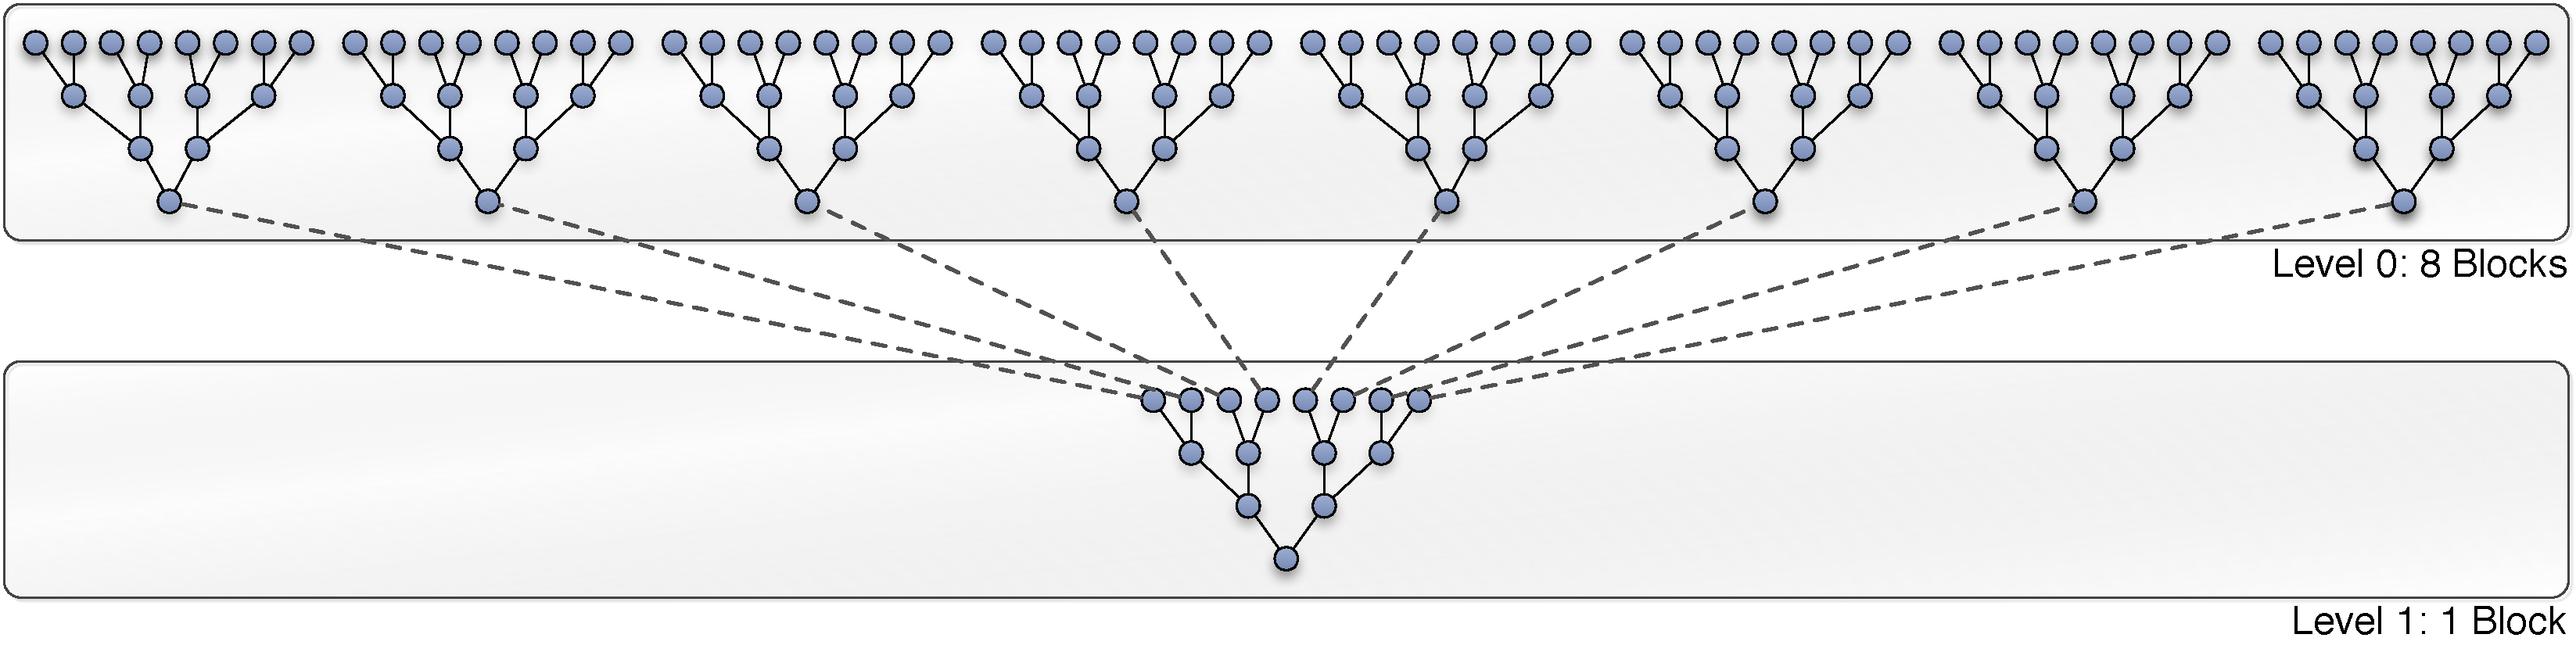
\includegraphics[width=\textwidth]{images/sec-4/tree-reduction}
    \end{center}
    \caption[A parallel tree reduction]{Illustration of a tree reduction,
        performed in two steps. In the first step 8 thread blocks in parallel
        reduce 8 elements to a single value. The thread blocks synchronise by
        writing their result to memory, and the kernel is called recursively
        until the final result is computed.}
    \label{fig:tree_reduction}
\end{figure}

For a fused dot product kernel, only the first line of reductions at level zero
perform the element wise multiplication. All subsequent reductions in that
kernel, as well as the recursive steps at level one and beyond, are pure
reductions. Thus, the fused operation requires compilation of two separate
kernels. % We focus on the level zero kernel, which is more interesting.

\subsubsection{Parallel Reduction Complexity}
\label{sec:parallel_reduction_complexity}

If each thread combines two elements at a time, then a vector of length $N$ will
\marginnote{tk: for power-of-2 n, add upper/lower bounds symbols}
be reduced in $\mathcal{O}\left( \log N \right)$ parallel steps. Each step $S$
does $\sfrac{N}{S^2}$ independent operations, so the \emph{step
complexity}\index{complexity!step} of the algorithm is:
\[
\mathcal{O}\left( \log N \right)
\]
For $N=2^{D}$, the algorithm thus performs $\sum_{S=1}^{D}2^{D-S} = N - 1$
operations. This means that the \emph{work complexity}\index{complexity!work} of
the algorithm is:
\[
\mathcal{O}\left( N \right)
\]
and so does not perform more work than a sequential algorithm. For $P$ threads
running physically in parallel on $P$ processors, the \emph{time
complexity}\index{complexity!time} is $\mathcal{O}\left( \sfrac{N}{P} + \log N
\right)$. In a thread block $N = P$, so the time complexity is:
\[
\mathcal{O}\left( \log N \right)
\]
Compare this to a sequential reduction, which has a time complexity of
$\mathcal{O}\left( N \right)$.

\subsubsection{Algorithm Cascading}
\label{sec:algorithm_cascading}

The \emph{cost} of a parallel algorithm is the number of processors $\times$
time complexity. This implies that the cost of the algorithm is
$\mathcal{O}\left( N \log N \right)$, which is \emph{not} cost efficient.

Brent's theorem~\cite{Chatterjee:2009vh} suggests that instead of each thread
summing two elements, \emph{algorithm cascading} can be used to combine a
sequential and parallel reduction. Each thread does $\mathcal{O}\left( \log N
\right)$ sequential work, which reduces the cost of the algorithm to
$\mathcal{O}\left( \sfrac{N}{\log N} \log N \right)$, or rather:
\[
\mathcal{O}\left( N \right)
\]
while keeping the work complexity $\mathcal{O}\left( N \right)$ and step
complexity $\mathcal{O}\left( \log N \right)$.

This suggests, for example, that a block of 256 threads should sum a total of
2048 elements. In practice it is beneficial to do even more sequential work per
thread, since this reduces the number of levels in the recursive tree reduction
and provides better latency hiding.


\subsubsection{Mapping to CUDA Threads}

Reduction of a one dimensional array uses multiple thread blocks to
cooperatively reduce the array, as described above. The number of thread blocks
is limited to the maximum number of blocks that can be simultaneously resident
on the current device, which requires that blocks each do a larger amount of
sequential work before beginning the cooperative reduction phase. This limits
the total kernel startup cost associated with launching thread blocks. Since the
maximum number of resident blocks is typically much less than the number of
threads in a block, the reduction will typically require at most two kernel
invocations.\footnote{Accelerate selects the thread block size in order to
maximise thread occupancy. As this depends on both the specific \GPU\ being used
as well as the user function the array is reduced with, an upper bound of two
parallel steps can not be guaranteed.}

Higher-dimensional reductions reduce the array along the innermost dimension
only. This is similar to a segmented fold, except that the segment descriptor is
not necessary since the length of every segment is the same and can be
determined from the array shape. Instead of thread blocks cooperatively reducing
each segment sequentially, each segment is reduced by a single thread block
which operates independently of all other thread blocks. A consequence of this
is that proper device utilisation depends on the shape of the array and not
simply the total number of elements in the array. For example, reduction of an
array with shape \code{(Z :. 1 :. n)} will use a single thread block, no matter
how large \code{n} is. This simplifies the implementation but is clearly not
always ideal.\footnote{The number of multiprocessors on a device various between
architecture generation and performance of a given card. For example, a Tesla
T10 processor (compute compatability 1.3) has 240 cores split over 30
multiprocessors, while a Kepler K20X processor (compute capability 3.5) has 2688
cores split over only 14 multiprocessors. A given architecture generation will
have the same number of cores per multiprocessor, and lower performance
processors in a generation are produced by incorporating (or activating) fewer
multiprocessors, thereby reducing the total core count.}

A segmented reduction uses a single warp to reduce each segment. Investigation
of whether it is be better to utilise a thread block per segment instead, or
convert the multidimensional reduction to this warp per segment strategy, is
left for future work.


\subsection{Scan}

Parallel scan and segmented scan algorithms are a crucial building block for a
great many data-parallel algorithms~\cite{Blelloch:1990ts,Chatterjee:1990vj}.
They also form the basis for efficiently mapping nested data-parallel languages
such as NESL~\cite{Blelloch:1995ut,Blelloch:1996jx} on to flat data-parallel
machines. Because of their fundamental importance to many algorithms,
implementing efficient scan operations in \CUDA\ has received much
attention~\cite{Sengupta:2007tc,Dotsenko:2008fo,Harris:2012fy}.

A basic description (in pictures) of how the scan and segmented scan algorithms
work.


\subsection{Permute}

The \code{permute} collective operation defines a forward permutation $f$ as an
index mapping from one array $X$ onto the result array $Y$, which we can write
as  $f : X \rightarrow Y$. Implementation of the permute function in Accelerate
is complicated because we have not placed any particular restrictions on $f$,
namely:
%
\begin{enumerate}
    \item $f$ is not surjective: the range of $f$ may not cover the codomain
        $Y$. For every $x$ in $X$, $f\left( x \right)$ need not yield every
        index $y$ in $Y$. This means that the result array must first be
        initialised with a set of default values.

    \item $f$ is not injective: distinct elements of the domain may
        map to the same element in the codomain. For all $x$ and $x'$ in $X$, if
        $f\left( x \right) = f\left( x' \right)$, we may have that $x \ne x'$.
        This means we require an associative combination function to combine
        elements from the domain that map to the same index in the codomain.

    \item $f$ is partial: elements of the domain may be ignored, and thus do
        not map to elements in the codomain.
\end{enumerate}

That the permutation function admits partial functions in the index mapping is
not particularly challenges for the implementation, and indeed is useful for
implementing the \code{filter} operation, shown in Listing~\ref{lst:filter}. The
special value \code{ignore} is used to drop elements of the input vector that do
not satisfy the predicate, by not mapping those indices to an index in the
codomain.
%
\begin{lstlisting}[style=haskell
    ,label=lst:filter
    ,caption={[Filter in Accelerate] Filtering returns only those elements of a
    vector which satisfy a predicate. This operation is included as part of
    Accelerate's standard prelude.}]
filter :: Elt a => (Exp a -> Exp Bool) -> Acc (Vector a) -> Acc (Vector a)
filter p vec
  = let flags            = map (boolToInt . p) vec
        (targetIdx, len) = scanl' (+) 0 flags
        defaults         = backpermute (index1 $ the len) id vec
    in
    permute const defaults (\ix -> flags!ix ==* 0 ? (ignore, index1 $ targetIdx!ix)) vec
\end{lstlisting}

On the other hand, because we can not prove that \code{filter} is surjective, we
require the result vector to be first initialised with default values. Since we
do not know anything about the element type \code{a}, the only recourse is to
copy elements from the input array \code{vec}. This is doubly wasteful, because
we must first execute the \code{backpermute} kernel to compute the
\code{defaults} array, and then copy those values into the results vector before
executing the \code{permute} kernel, even though we know the initialised values
will be completely overwritten.

At a second example, Listing~\ref{lst:histogram} demonstrates the computation of
a simple ten bin histogram from a vector of floating point elements in the range
$\left[ 0, 100 \right)$. In this case the permutation function is neither
surjective nor injective, as some bins may contain no elements and thus take the
default value, while other bins may contain multiple elements which need to be
combined (accumulated) correctly.
%
\begin{lstlisting}[style=haskell
    ,label=lst:histogram
    ,caption={[Simple histogram in Accelerate] A simple histogram written in
    Accelerate. We assume the input vector contains elements in the range
    $\left[0,100\right)$ and accumulate into ten equally sized bins.}]
histogram :: Acc (Vector Float) -> Acc (Vector Int)
histogram vec
  = let bins      = 10
        zeros     = fill (constant (Z :. bins)) 0
        ones      = fill (shape vec)            1
    in
    permute (+) zeros (\ix -> index1 (A.floor ((vec ! ix) / P.fromIntegral bins))) ones
\end{lstlisting}

The semantics of the operation is that every permutation from source to result
array is applied at the same time in a single parallel step. If multiple \CUDA\
threads attempt a non-atomic write to the same memory location at the same time,
the writes will be serialised but the thread which performs the final write is
undefined, and so the final value at that memory slot is
undefined~\cite{NVIDIA:2012wf}. To support non-injective permutation functions,
which is required to evaluate the histogram program correctly, the atomic
compare-and-swap operation is used to implement write combining.\footnote{The
atomic compare-and-swap operation on 32-bit values is only available for devices
of compute capability 1.1 and higher, and for 64-bit values on devices of
compute capability 1.2 and higher.} For a combination function \code{f} on
elements of type \code{T}, the following atomically combines a value from the
source array \code{x} with the value of the result array \code{y}.

\begin{lstlisting}[style=cuda]
    T x         = source[i];
    T y, old_y  = result[j];
    do {
        y       = old_y;
        old_y   = atomicCAS(&result[j], y, f x y);
    } while (y != old_y);
\end{lstlisting}
%
Any atomic operation on simple types can be implemented in terms of
compare-and-swap in this manner. Types consisting of more than one primitive
type, such as tuples, apply the procedure to each component separately.
Utilising more specific atomic operations such as \code{atomicAdd} when
available is left to future work.

\subsection{Stencil}


\section{Memory Management}
\label{sec:memory_management}

In a standard Haskell program, memory is managed entirely automatically by the
runtime system. This relieves a large burden from the programmer and eliminates
a source of potential runtime errors. In contrast, in the \CUDA\ programming model
all memory management is explicit and handled by the programmer. Indeed, \CUDA\
devices typically have their own memory, physically separate from the memory of
the host CPU, which data must be explicitly transferred to and from.

In order to keep Accelerate programs as close to idiomatic Haskell as possible,
the Accelerate runtime system should do the job of managing the \CUDA\ memory
space. Moreover, host-device data transfers are expensive, given the relatively
high latency and low bandwidth of the PCI-E bus, so minimising data transfer is
an important pressure point for achieving high performance. There are several
considerations in order to realise this.

% The question is (a) when should data be transferred to and from the host, to be
% made available for CPU and GPU computations respectively; and (b) when should
% arrays on the GPU be allocated and deallocated.


\subsection{Device-to-host transfers}

Evaluating Accelerate expressions is done with the following function, which
encapsulates the entire process of compiling and executing a program on the
\GPU\ (\S tk):
%
\begin{lstlisting}[style=haskell,numbers=none]
    run :: Arrays a => Acc a -> a
\end{lstlisting}
%
The result of evaluating this program is made available for use in vanilla
Haskell, so \code{run} must copy the final array result back to the host.
However, any intermediate results computed during evaluation of the program are
\emph{not} copied back to the host.


\subsection{Host-to-device transfers}
\label{sec:host_device_transfers}

Accelerate distinguishes between vanilla Haskell arrays (in CPU host memory)
from embedded arrays (in \GPU\ device memory). Every array on the host is
uniquely associated to an array on the device, which defines where data is
copied when data is transferred between the host and device. The function
\code{use} embeds a Haskell array into an embedded array computation, and thus
implies host-to-device data transfer:
%
\begin{lstlisting}[style=haskell,numbers=none]
    use :: Arrays arrays => arrays -> Acc arrays
\end{lstlisting}
%
% The \code{Arrays} class constrains the type to either a single array of type
% \code{Array sh e}, where \code{sh} and \code{e} characterise the types that may
% be used as array indices and elements respectively, or a tuple of arrays (see \S
% tk).

At a first approximation, we simply copy the data to the \GPU\ as soon as we
encounter the \code{Use} node in an expression. This occurs during the first
phase of program execution, and is done asynchronously\footnote{Testing reveals
that the data transfer does not in fact occur asynchronously, and fixing this is
left for future work. See \S\ref{sec:memory_management_conclusion}.}
so that it may overlap code generation and compilation
(\S\ref{sec:dynamic_compilation}). However, we can do better.

\subsubsection{Intra-expression sharing}

Consider the following example, where we \code{use} a single array twice. Since
Accelerate operations are pure and thus do not mutate arrays, the device arrays
can be safely shared. Thus, we would like these two arrays to refer to the same
data in \GPU\ memory. This reduces the amount of memory required to store the
data as well as reducing memory traffic.\footnote{Why doesn't sharing recovery
(\S\ref{sec:sharing_observation}) notice that the two uses of \footcode{xs} are
the same and combine them? The sharing recovery algorithm observes the sharing
of \emph{Accelerate} terms, and because we have called \footcode{use} twice, we
are effectively constructing two \emph{separate} Accelerate terms
(\footcode{Use} nodes). Furthermore, since GHC does not do common subexpression
elimination, as it can affect the strictness/laziness of the program and
potentially introduce space leaks
(\url{http://ghc.haskell.org/trac/ghc/ticket/701}), these common subexpressions
are not combined, two separate values are created on the heap, and there is no
sharing to be observed.}
%
\begin{lstlisting}[style=haskell]
square :: (Elt e, IsNum e, Shape sh) => Array sh e -> Acc (Array sh e)
square xs = zipWith (*) (use xs) (use xs)
\end{lstlisting}

Since the two \code{use} nodes refer to the same array on the heap, they will
share the same array in \GPU\ memory, and thus the data is only copied once.
This is a happy consequence of way we uniquely associate host and device arrays.


\subsubsection{Inter-expression sharing}

At a second example, consider the following program fragment, which given an
array describing the particle density \code{df} and the direction and magnitude
of the velocity field \code{vf} at each point, computes how the density and
velocity fields evolve under advection and diffusion:
%
\begin{lstlisting}[style=haskell]
fluid :: Timestep                               -- time to evolve the simulation
      -> Viscosity                              -- viscous damping factor
      -> Diffusion                              -- mass diffusion rate
      -> Acc DensityField                       -- particle densitey at each point in the field
      -> Acc VelocityField                      -- velocity at each point in the field
      -> Acc (DensityField, VelocityField)
fluid dt dp dn df vf =
  let vf'       = velocity steps dt dp vf       -- dampen velocity field
      df'       = density  steps dt dn vf' df   -- move particles based on forces
  in
  A.lift (df', vf')
\end{lstlisting}
%
This is the entry function to the program that implements Jos Stam's stable
fluid algorithm~\cite{Stam:1999ey} (\S\ref{sec:fluid}). As is typical with
numerical simulations, to evolve the simulation over a period of time the
function is called repeatedly over small time steps, with the output of each
step of the simulation forming the input to the next. That is, given some
initial values \code{df0} and \code{vf0} the simulation proceeds as:
%
\begin{lstlisting}[style=haskell]
simulation dt dp dn df0 vf0 =
  let (df1, vf1)        = run $ fluid dt dp dn df0 vf0  -- first step using initial conditions
      (df2, vf2)        = run $ fluid dt dp dn df1 vf1  -- second step progresses result of the first
      (df3, vf3)        = run $ fluid dt dp dn df2 vf2  -- \ldots and so on
      ...
\end{lstlisting}
%
Thus, the results of the first step \code{df1} and \code{vf1} will be the inputs
to the second step of the simulation, and so on. Since these arrays were just
copied \emph{from} the \GPU, we should avoid immediately copying the \emph{same
data} back again in the subsequent step.

To be able to avoid this redundant transfer, the Accelerate memory manager needs
to operate over the lifetime of the entire Haskell program, and not be
constrained to work within a single \code{run} invocation. Otherwise, all device
memory needs to be deallocated after evaluating the expression, or the program
will leak memory. Thus, localised memory management techniques such as reference
counting or syntax directed allocations are insufficient.

The key observation is that the Haskell runtime system knows when objects will
be reused (the result of the first step \code{df1} is used in the second step),
and when they are no longer required and can be garbage collected (\code{df1} is
no longer needed after evaluating the second step and can be safely
deallocated). Since every array in \GPU\ memory is uniquely associated with an
array on the host, which is managed by the Haskell runtime system, we attach
finalisers~\cite{PeytonJones:2000ks} to the host array which deallocate the
\GPU\ memory at the same time the Haskell heap object is garbage collected.

% To be
% precise, since the CUDA backend uses a hash table to record the associations
% between host and device arrays, we construct a weak hash
% table~\cite{PeytonJones:2000ks}, so that entries can both deallocate the device
% memory as well as remove themselves from the association table when the array is
% garbage collected, and so that all finalisers can be initiated immediately if
% the hash table is itself is garbage collected.
% 
% \note{This section was very handwavey. Introduce actual types/code for the core
% memory table operations.}


\subsection{Allocation \& Deallocation}

The Accelerate language defines only pure operations on arrays, so every kernel
stores its result into a fresh device array. This style of programming results
in a very high memory allocation and deallocation rate. For programs that
execute many kernels, such as the fluid simulator, this can have a
significant contribution to overall performance (\S\ref{sec:fluid}).

Instead of immediately deallocating device memory when an array is garbage
collected, we instead remove its association to a specific host array but retain
a reference to the device memory for later reuse. This memory area is the
\indexe{nursery}, which is simply a finite mapping from array sizes to a chuck
of memory of that size. When a new array is allocated, we first check if a block
of the appropriate size is available in the nursery; if so that block is reused,
else fresh memory is allocated.

% To increase the hit rate of the nursery, allocations for fresh arrays are
% rounded up to a set chunk size, rather than being sized to exactly fit the
% required number of elements. If an allocation for fresh data fails due to
% insufficient memory, data held by the nursery is immediately deallocated and the
% fresh allocation reattempted.
% 
% \begin{lstlisting}[style=haskell]
% type NRS        = IORef ( HashTable (Context, Int) (FullList () (DevicePtr ())))
% type Nursery    = Nursery NRS (Weak NRS)
% \end{lstlisting}

\subsection{Memory manager implementation}

The memory management system is implemented over several modules:
%
\begin{description}
\item[Data] Defines operations on the surface \code{Array} data type, in
    particular applying operations to each member of the struct-of-array
    representation.

\item[Prim] Interface to the \CUDA\ API for operations on arrays of primitive
    type, for example to initiate data transfers to and from the device. Queries
    the memory table functions to retrieve the raw pointers for device arrays.

\item[Table] Maps host arrays to the corresponding array in device memory, and
    sets up finalisers so device arrays can be moved into the nursery when the
    host array is garbage collected.

\item[Nursery] Handles allocation and deallocation of device memory, and
    manages unused blocks of memory that can be reused instead of allocating
    fresh data.
\end{description}

Implementation of the Data and Prim modules is not extraordinary, but it is
worthwhile mentioning that care should be taken with the implementation of
transferring an array to the device via \code{use}. In particular, that the
array data is only transferred on the first \code{use} attempt, when a fresh
device array was allocated. If the \code{use} operation is separated into its
constituent \code{malloc} and \code{poke} operations, this is easily overlooked
resulting in the array data being needlessly transferred every time \code{use}
is called.

The \emph{memory table} records the association between host and device arrays.
Implemented as a weak hash table~\cite{PeytonJones:2000ks}, the table can purge
itself of unneeded key/value pairs, releasing the device memory at the same time
by moving it to the nursery. Furthermore the table will also release itself when
no longer required, initialising the finalisers for all key/value pairs as it
goes.
%
\begin{lstlisting}[style=haskell]
type MT                 = IORef ( HashTable HostArray DeviceArray )
data MemoryTable        = MemoryTable MT (Weak MT) Nursery

data HostArray where
  HostArray   :: exists e. Typeable e
              => CUDA.Context                   -- a specific device execution context
              -> StableName (ArrayData e)       -- array data on the host CPU
              -> HostArray

data DeviceArray where
  DeviceArray :: exists e. Typeable e
              => Weak (DevicePtr e)             -- data on the GPU
              -> DeviceArray
\end{lstlisting}
%
The key and value parts of the hash table are packaged into untyped containers
so that all arrays are tracked using a single memory table. The \code{Typeable}
constraint permits a type-safe cast to later recover the existentially
quantified array type. Furthermore the host arrays are tagged with a specific
\CUDA\ context, which is used to support mapping the host array to multiple
devices and execution contexts. Looking up an array in the memory table
demonstrates the procedure for working with weak pointers.
% The implementation of the lookup operation follows closely that of
% \citet{PeytonJones:2000ks}.
%
\begin{lstlisting}[style=haskell]
lookup :: (Typeable a, Typeable b)
       => Context
       -> MemoryTable
       -> ArrayData a
       -> IO (Maybe (DevicePtr b))
lookup ctx (MemoryTable ref _ _) arr = do
  sa <- makeStableArray ctx arr                                         -- (1)
  mw <- withIORef ref (`HashTable.lookup` sa)
  case mw of
    Nothing              -> return Nothing
    Just (DeviceArray w) -> do                                          -- (2)
      mv <- deRefWeak w
      case mv of
        Just v | Just p <- gcast v -> return (Just p)
               | otherwise         -> error "lookup: type mismatch"
        Nothing                    -> do                                -- (3)
          sa' <- makeStableArray ctx arr
          error ("lookup: dead weak pair: " ++ show x)
\end{lstlisting}
%
\begin{enumerate}
\item The memory table maps a stable name of the argument host-side array to a
    weak pointer to the corresponding device array of a given context.

\item If the lookup is successful, we can attempt to dereference the weak
    pointer to find the actual value. On success, A type-safe cast is used to
    recover the existentially quantified type of the array data.

\item However there is an awkward race condition here, because at the moment
    \code{deRefWeak} is called there might, conceivably, be no further
    references to the host array \code{arr}. If that is so, and a garbage
    collection intervenes, the weak pointer might be tombstoned before
    \code{deRefWeak} gets to it. In this unusual case we throw an error, but in
    doing so this makes \code{arr} reachable in the continuation of
    \code{deRefWeak}, and thus ensures \code{deRefWeak} will always succeed.
    This sort of weirdness, typical of the world of weak pointers, is why we can
    not reuse the stable name \code{sa} computed above in the error message.
\end{enumerate}

The nursery is a hash table from array sizes to a non-empty list of pointers to
arrays of that size. Keys are additionally tagged with the device execution
context within which they are allocated.
%
\begin{lstlisting}[style=haskell]
type NRS        = IORef ( HashTable (CUDA.Context, Int) (FullList () (DevicePtr ())) )
data Nursery    = Nursery NRS (Weak NRS)
\end{lstlisting}
%
Querying the nursery returns a pointer to an array of the given size if one is
available, removing it from the nursery. If no suitably sized chunks are
available, fresh memory needs to be allocated instead.
%
\begin{lstlisting}[style=haskell]
malloc :: forall a b. (Typeable a, Typeable b, Storable b)
       => Context
       -> MemoryTable
       -> ArrayData a
       -> Int
       -> IO (DevicePtr b)
malloc ctx mt@(MemoryTable _ _ nursery) ad n = do
  let multiple x f      = floor ((x + (f-1)) / f :: Double)             -- (1)
      chunk             = 1024
      n'                = chunk * multiple (fromIntegral n) (fromIntegral chunk)
      bytes             = n' * sizeOf (undefined :: b)
  --
  mp  <- Nursery.malloc bytes (deviceContext ctx) nursery               -- (2)
  ptr <- case mp of
           Just p       -> return (CUDA.castDevPtr p)
           Nothing      ->
             CUDA.mallocArray n' `catch` \(e :: CUDAException) ->       -- (3)
               case e of
                 ExitCode OutOfMemory -> reclaim mt >> CUDA.mallocArray n'
                 _                    -> throwIO e
  insert ctx mt ad ptr bytes                                            -- (4)
  return ptr
\end{lstlisting}
%
\begin{enumerate}
\item Instead of allocating the array size to be exactly as many elements as
    needed, round up to the next highest multiple of a set chunk size. This
    improves the reuse rate for the nursery.

\item Check the nursery if a block of the right size can be reused. This avoids
    calling out to the \CUDA\ API to allocate fresh data, which must pause until
    any currently executing kernels complete.

\item If nothing is available from the nursery, allocate a new array. If this
    fails, attempt to recover any free memory by running any pending finalisers
    and clearing the nursery, then try again.

\item Update the memory table with this new host/device array association.

\end{enumerate}

Finally, we present the finaliser that is invoked when the host array is garbage
collected by the Haskell runtime. The finaliser refers to its surrounding
execution context via weak pointers, otherwise these values will be kept alive
until all keys have become unreachable.
%
\begin{lstlisting}[style=haskell]
finalizer :: Weak CUDA.Context          -- execution context this array is allocated in
          -> Weak MT                    -- memory table
          -> Weak NRS                   -- nursery
          -> HostArray -> DevicePtr b   -- key/value pair
          -> Int                        -- array size in bytes
          -> IO ()
finalizer weak_ctx weak_tbl weak_nrs key ptr bytes = do
  mr <- deRefWeak weak_tbl                                              -- (1)
  case mr of
    Nothing  -> return ()
    Just tbl -> withIORef tbl (`HashTable.delete` key)
  --
  mc <- deRefWeak weak_ctx                                              -- (2)
  case mc of
    Nothing  -> return ()
    Just ctx -> do
      mn <- deRefWeak weak_nrs                                          -- (3)
      case mn of
        Nothing  -> bracket_ (CUDA.push ctx) CUDA.pop (CUDA.free ptr)
        Just nrs -> Nursery.stash bytes ctx nrs ptr
\end{lstlisting}
%
\begin{enumerate}
\item If the memory table is still alive, remove this association between host
    and device arrays.

\item If the \CUDA\ execution context has been garbage collected, then the
    device memory has implicitly been deallocated already and there is nothing
    further to do.

\item Otherwise, if the nursery is still active stash the array there for
    possible later reuse, otherwise deallocate it immediately. Note that since
    the finaliser might run at any time, we need to reactivate this specific
    context for the duration of the deallocation.
\end{enumerate}


\subsection{Conclusion}
\label{sec:memory_management_conclusion}

The Accelerate runtime automatically manages the \CUDA\ memory space through the
use of finalisers to hook in into the garbage collector of the runtime system of
the host program. The system is able to avoid several types of redundant data
transfer between the host CPU and attached \GPU\, which is important for
achieving high performance.

The amount of memory available on the device often limits the size of problems
that the \GPU\ can be used to solve. The current system is designed to minimise
host-device memory transfers, which can increase the lifetime of arrays stored
on the device. Future work could improve handling of programs which exceed the
available memory, for example in the case where this is due to the use of many
intermediate or input arrays, but where individual sub-problems fit within the
available memory. In this case arrays that are not required for the current
calculation can be evacuated from the device by transferring back to the
associated host-side array, and transferred back to the device only once
required.

While it is possible to overlap memory transfers with both kernel executions and
tasks such as compilation and optimisation, the current implementation does not
completely implement this. To support asynchronous memory transfer requires the
use of non-default streams and event waiting, the same as required for
concurrent kernel execution (\S tk). Additionally, the array on the host needs
to be \emph{page-locked} or \emph{pinned} so that it can be accessed directly by
the \GPU\ using direct memory access (DMA). Regular memory allocations are
\emph{pageable} by default, which means the host operating system is free to
change the physical location of the data, such as moving the data to disk in
order to free up memory for other applications. Since the location of pageable
memory can change, and may not exist in physical RAM at all, this memory can not
be directly accessed by the \GPU\@. Instead when copying data to the \GPU\ from
pageable memory, the \CUDA\ library must first copy the data to a staging area
allocated using pinned memory, and then transfer the data to the device from the
staging area. Only the second step of this process proceeds asynchronously.
Allocations on the host are currently handled by the core Accelerate package,
which contains no \CUDA\ specific operations such as using pinned\footnote{The
memory allocated by Accelerate is pinned only with respect to the Haskell
garbage collector, not with respect to the host operating kernel. Regardless,
the \CUDA\ runtime maintains its own notion of pinned memory separate from the
kernel notion of pinned memory as specified using \footcode{mlock()}.} memory.
Note that page-locked memory is a scarce resource and reduces the amount of
physical memory available to the operating system, so consuming too much
page-locked memory can reduce overall system performance~\cite{NVIDIA:2012wf}.


\section{Skeleton-based code generation}
\label{sec:code_generation}

\subsection{Scalar code}
\subsection{Shapes}
\subsection{Tuples}
\subsection{Array references in scalar code}


\section{Dynamic Compilation}
\label{sec:dynamic_compilation}

When you write a program in Accelerate, what you are really doing is writing a
Haskell program that \emph{generates} a \CUDA\ program, that is compiled,
loaded, and executed on the \GPU\@. Thus, one major difference between using
Accelerate for general purpose \GPU\ programming compared to programming in
\CUDA\ directly, is that kernels are generated dynamically, at application
\emph{runtime}, whereas plain \CUDA\ code is pre-compiled.

Dynamic code generation has significant advantages, especially for embedded
languages. In particular, the code generator can query the capabilities of the
hardware on which the code will be executed, and optimise the generated program
accordingly, as well as specialise the code to the available input data. The
host program can also be used to generate the embedded program.

The main drawback of dynamically generating and compiling \GPU\ kernels is the
additional execution time required to do so, so attempts must be made to
mitigate these overheads. In general purpose \GPU\ programming, it is only
worthwhile to offload computations to the \GPU\ if they are computationally
intensive. This implies a significant runtime and usually also the use of
significant amount of input and/or output data. Hence, the overhead of dynamic
kernel compilation is not necessarily problematic in the face of long kernel
runtimes and long data-transfer times between host and device memory, especially
if those kernels are compiled once and executed on multiple data sets.

\subsection{External compilation}
\label{sec:external_compilation}

In unison with the \AST\ traversal that extracts \code{Use} subterms to initiate
data transfers (\S\ref{sec:host_device_transfers}), the \CUDA\ backend initiates
code generation for each collective array operation it encounters via skeleton
instantiation (\S\ref{sec:code_generation}). After the \CUDA\ code is generated,
it must be compiled with the external \texttt{nvcc} tool-chain to produce binary
object code for the kernels implementing each collective operation.

As with data transfer, the compilation of the generated \CUDA\ code proceeds
asynchronously, and linking of the compiled code is deferred until it is needed
during execution. For each generated kernel, the \CUDA\ compiler is invoked by
spawning an external process that executes the raw system command. However, if
the program requires the compilation of many kernels, carelessly spawning a new
process for every instantiated skeleton can cause the IO bus to become
saturated, further increasing compilation time, or exhaust the host operating
system's available process handles. To counter this problem, a worker pool is
created that will be used to process jobs in first-in first-out (FIFO) order:
%
\begin{lstlisting}[style=haskell]
{-# NOINLINE worker #-}
worker :: Queue.MSem Int
worker = unsafePerformIO $ Queue.new =<< getNumProcessors
\end{lstlisting}

The worker pool is defined as the Haskell equivalent of a global
variable\footnote{The idiom popularly known as ``the unsafePerformIO hack''.}
and is initialised once per program execution. The number of slots in the queue
is set to the number of physical CPU cores present in the host
system\footnote{Note that this is not limited by the RTS option \texttt{-N} that
specifies the number of processors to use.} which specifies the maximum number
of kernels to compile concurrently. Instead of initiating the compilation
process directly, it is instead added to the work queue:
%
\begin{lstlisting}[style=haskell,firstnumber=last]
enqueueProcess :: FilePath -> [String] -> IO (MVar ())
enqueueProcess nvcc flags = do
  mvar  <- newEmptyMVar                                         -- (2)
  _     <- forkIO $ do                                          -- (1)
    Queue.with worker $ do                                      -- (3)
        (_,_,_,pid)     <- createProcess (proc nvcc flags)
        waitFor pid
    --
    putMVar mvar ()                                             -- (4)
  --
  return mvar
\end{lstlisting}

\begin{enumerate}
\item The process is spawned from a separate thread so that the thread can block
    waiting for both the worker queue and the external process, without
    interrupting the main thread. Thus compilation proceeds asynchronously with
    outer host processing tasks.

\item An empty \code{MVar} is created that will act as a signal to the main
    thread that the external process has completed. Since \code{takeMVar} on an
    empty \code{MVar} blocks until that \code{MVar} is filled, the main thread
    can wait for the external process to complete if the compiled code is not
    yet available by the time it is required during the execution phase.

\item The thread waits for a worker to become available from the queue. Blocked
    threads are woken up by the runtime system and are serviced in a first-in
    first-out order; that is, threads do not actively poll the queue continually
    testing for an open slot. Once a worker becomes available, the external
    process is launched and the thread once again blocks until that process
    completes.

\item Once the process completes the worker is returned to the queue where it
    can be assigned to handle any further tasks. Finally, the thread fills the
    \code{MVar} to signal the main thread that the compilation has completed.
\end{enumerate}

We return to the question of linking in the compiled code below, when we discuss
the process of executing the program.


\subsection{Caching compiled kernels}
\label{sec:caching_compiled_kernels}

The \CUDA\ backend associates each \CUDA\ binary with the skeleton instantiation
whose computation that binary implements. Furthermore, the binary object code is
keyed on a skeleton and the parameters of its instantiation, not to the specific
AST node used to instantiate the skeleton. As a result, compiled binaries are
reusable when the same skeleton instantiation is required again, whether that is
in the same Accelerate computation applied to a different set of input arrays,
or an entirely different computation. For example, operations such as
\code{scanl (+) 0} are common, and it would be wasteful to dynamically generate
and compile the same code multiple times.

\begin{lstlisting}[style=haskell,numbers=none]
type ProgramCache = HashTable KernelKey KernelEntry

type KernelKey = (CUDA.Compute, ByteString)
data KernelEntry
    = CompileProcess FilePath (MVar ())                                 -- (1)
    | KernelObject ByteString (FullList CUDA.Context CUDA.Module)       -- (2)
\end{lstlisting}

The cache is a hash table which is keyed by an MD5~\cite{Rivest:1992va} digest
of the generated \CUDA\ code which instantiates the skeleton, as well as the
compute capability the generated code was specialised and compiled for. The hash
table value can either refer to:
%
\begin{enumerate}
\item A currently compiling external process. This records the path of the file
    currently being compiled, which will be rooted in a temporary directory, as
    well as the \code{MVar} that will signal when the external process has
    completed (\S\ref{sec:external_compilation}). If a kernel is requested that
    is currently compiling, the thread blocks on the \code{MVar} until the
    result is available and then updates the hash table with;

\item The raw compiled data with a non-empty list of \CUDA\ contexts that the
    object code has been linked into. The entry may have been added to the cache
    by an alternate context of the same compute capability, for example on a
    system with multiple \CUDA\ devices, so the code simply needs to be
    re-linked for the current context.
\end{enumerate}

This scheme effectively caches kernels both within the same Accelerate
computation and across different Accelerate expressions. However, it must be
regenerated ever time the program is executed, which increases program startup
time. Once a kernel is compiled, the binary object code is saved in the user's
home directory so that it is available across separate runs of the program, or
indeed different programs. This information is stored in a persistent cache:
%
\begin{lstlisting}[style=haskell,numbers=none]
type PersistentCache = HashTable KernelKey ()
\end{lstlisting}

The persistent cache is a hash table indexed by the same key used by the
in-memory cache described above, but without a value component. Instead, the
presence of a key in the persistent cache indicates that the compiled binary
represented by that key is available to be loaded from disk. The location of the
object code is determined from the MD5 digest by creating a ASCII representation
of the digest, replacing special characters with z-encoded strings.
%
\begin{lstlisting}[style=haskell]
encode_ch :: Char -> String
encode_ch c | unencodedChar c = [c]             -- regular characters except `z' and `Z'
encode_ch '('  = "ZL"                           -- punctuation using two-character sequences
encode_ch ')'  = "ZR"
  ...
encode_ch c    = encode_as_unicode_char c       -- other characters using hexadecimal
\end{lstlisting}

Initialising the persistent cache populates the hash table by reading an index
file from disk, which is simply a binary file containing the number of entries
at the start of the file, followed by the keys.
%
\begin{lstlisting}[style=haskell]
restore :: FilePath -> IO PersistentCache
restore db = do
  exist <- doesFileExist db
  case exist of
    False       -> encodeFile db (0::Int) >> HashTable.new
    True        -> do
      store         <- L.readFile db
      let (n,rest,_) = runGetState get store 0
      pt            <- HashTable.newSized n
      --
      let go []      = return ()
          go (!k:xs) = HashTable.insert pt k () >> go xs
      --
      go (runGet (getMany n) rest)
\end{lstlisting}

The \texttt{binary} package is used to deserialise the data from file. Note that
the implementation for serialising lists of elements provided by that preserves
the order of elements in the list, which requires creating the entire list
structure in memory.\footnote{A tail-recursive loop that accumulates the list
structure as the file is read sequentially from disk produces list elements in
reverse order. Thus, the list must be reversed before being returned, making the
structure spine-strict and preventing elements being consumed as they are read
from file.} Since we do not require this property, we provide our own
deserialisation routine that allows the elements to be lazily consumed and added
directly to the hash table as they are read from file.

\begin{lstlisting}[style=haskell]
getMany :: Binary a => Int -> Get [a]
getMany n = go n []
  where
    go 0 xs = return xs
    go i xs = do x <- get
                 go (i-1) (x:xs)
\end{lstlisting}

Finally, we present the entire \emph{kernel table} data structure used to cache
compiled kernels, consisting of in-memory kernels tracked by the program cache
as well as the on-disk kernels tracked by the persistent cache.

\begin{lstlisting}[style=haskell]
data KernelTable = KT ProgramCache      -- first level, in-memory cache
                      PersistentCache   -- second level, on-disk cache
\end{lstlisting}

Looking for entries in the kernel table entails first search the in-memory
program cache, which represents kernels that are (a) currently compiling; (b)
compiled, but not linked into the current context; or (c) compiled and linked
into the current context. If the kernel is not available in the program cache,
the persistent cache is searched. If found, the associated object file is linked
into the current context, and the program cache is updated to include this
entry. Conversely, the persistent cache must be explicitly updated after each
new kernel is compiled; the current behaviour for adding entries to the kernel
table only updates the in-memory cache, and does not attempt to keep the two
caches synchronised.


\subsection{Executing programs}
\label{sec:executing_programs}

The previous sections discuss how to implement asynchronous compilation as well
as kernel caching in order to reduce the overheads of dynamic compilation. When
we wish to execute a collective array operation, we query the kernel cache for
object code instantiated to that skeleton; if no appropriate kernel is found
then new code is generated and compiled, asynchronously to other operations such
as transferring input data to the device. These tasks occur during the first
pass over the program AST.

Once code generation and array transfer have completed, the \CUDA\ backend
traverses the program AST once more, evaluating the entire program by executing
the generated GPU kernel(s) for each collective array operation of the AST
bottom-up. In order to do this efficiently, the first phase outputs a new AST
where each node is decorated with all of the information required to executed
that collective operation.% How is this achieved?

% BEGIN ASIDE {
Recall that terms in the Accelerate core language are defined non-recursively.
At an example, consider this definition of a binary tree, which store all data
at the leaves of the tree and is parameterised by the type of the leaf element:
%
\begin{lstlisting}[style=haskell]
data Tree a
    = Leaf a                            -- Leaves of the tree hold the data
    | Node (Tree a) (Tree a)            -- Internal nodes record only left and right branches
\end{lstlisting}
%
Note that the internal \code{Node}s of the \code{Tree} are defined in terms of
itself, recursively. Instead, the tree can be parameterised by the recursive
step:
%
\begin{lstlisting}[style=haskell,name=pretree]
data PreTree tree a
    | Leaf a
    | Node (tree a) (tree a)
\end{lstlisting}
%
and the original tree can be recovered from this definition, albeit with the
need to unwrap the \code{Tree} constructor before exposing the \code{Leaf} and
\code{Node} constructors of the tree itself:
%
\begin{lstlisting}[style=haskell,name=pretree]
data Tree a = Tree (PreTree Tree a)
\end{lstlisting}

This distinction is important because it allows us to use the same basic tree
definition, but include additional information as part of each recursive step.
For example, we can define a new binary tree type that records the size of the
subtree at each point, and any existing functions operating over the basic
\code{PreTree} structure can still be used:
%
\begin{lstlisting}[style=haskell,name=pretree]
data SizedTree a = SizedTree Int (PreTree SizedTree a)
\end{lstlisting}
% END ASIDE }

Accelerate uses this technique to decorate each node of the AST with all of the
information required to execute the skeleton(s) implementing that node.
Following the fusion transformation (\S\ref{sec:fusion}), the recursive step of
nodes in the AST are parameterised as either \code{Manifest} or \code{Delayed},
representing computations that will be instantiated to \CUDA\ code and executed,
and computations that have been fused (embedded) into other kernels
respectively. To execute a computation in the second phase, the former requires
information of the kernels implementing the computation as well as any free
variables, while the latter requires only the shape of the computation that was
embedded within the consumer. The following data structure is used to tie the
recursive knot in the program AST to represent this information:
%
\begin{lstlisting}[style=haskell]
data ExecOpenAcc aenv a where
  ExecAcc   :: FL.FullList () (AccKernel a)             -- (1)
            -> Gamma aenv                               -- (2)
            -> PreOpenAcc ExecOpenAcc aenv a
            -> ExecOpenAcc aenv a

  EmbedAcc  :: (Shape sh, Elt e)
            => PreExp ExecOpenAcc aenv sh               -- (3)
            -> ExecOpenAcc aenv (Array sh e)
\end{lstlisting}
%
\begin{enumerate}
\item A non-empty list of the kernels required to execute this node of the
    computation (see below).

\item The free array variables required to execute the kernel. In particular,
    this maps environment indexes (de Bruijn indices) to some token identifying
    that array in the generated code. Rather than using the de Bruijn index
    directly in the generated code, the extra indirection results in generating
    code that is less sensitive to the placement of let bindings, ultimately
    leading to better kernel caching.

\item The size of the input array that was embedded into the consumer, which is
    often required when executing a kernel.
\end{enumerate}

In order to execute a single kernel the following data is required:
%
\begin{lstlisting}[style=haskell]
data AccKernel a where
  AccKernel :: String -> CUDA.Fun -> CUDA.Module        -- (1)
            -> CUDA.Occupancy -> Int -> Int             -- (2)
            -> (Int -> Int)                             -- (3)
            -> AccKernel a
\end{lstlisting}
%
\begin{enumerate}
\item The name of the \code{\_\_global\_\_} kernel function that the function
    object (second parameter) implements. The compiled object code is linked
    into the \CUDA\ context as part of the binary module (third parameter).

    % The results of \CUDA\ thread occupancy calculation.
\item Once the kernel is compiled, details such as the number of registers
    required for each thread can be used to determine the optimal launch
    configuration of the kernel. In particular, the configuration is chosen in
    order to maximum \indexe{thread occupancy}, which is the ratio of active
    warps (i.e.\ warps that could run) to the maximum possible number of active
    warps. While higher occupancy does not always equate to higher performance,
    low occupancy always interferes with the ability to hide memory and
    instruction latency, resulting in sub-optimal performance. This analysis
    (fourth parameter) determines the optimal number of threads per block to use
    (fifth parameter) together with the number of bytes of shared memory
    required when initiating the kernel launch (sixth parameter).

\item A function that computes the number of thread blocks to launch the kernel
    with given the size of the computation, which is generally only known at
    program runtime. How this function is used exactly depends on the kernel
    being executed, but for example may take as input the size of the input
    array.
\end{enumerate}

This formulation does not require searching the kernel tables during the
execution phase in order to locate binary code; any kernels required to execute
a computation are attached directly to the computation they instantiate. For
Accelerate programs that are executed on multiple data sets, this is an
important optimisation, and is further exploited when executing embedded
Accelerate programs using the \code{run1} operator (see \S tk).

Note that there is a subtle tension here: the task of the compilation phase is
to produce an annotated AST carrying all of the information required to execute
the computation, but that in turn requires the \emph{compiled} kernel modules,
so how can compilation proceed asynchronously? We use a clever trick and take
advantage of Haskell's non-strict execution semantics: once the external
compilation has been initiated in a separate thread, \code{unsafePerformIO} is
used (in a safe manner) to delay waiting for the external process to complete
and linking of the binary object until it is demanded by the running program.
%
\begin{lstlisting}[style=haskell]
build1 :: DelayedOpenAcc aenv a -> CIO (AccKernel a)
build1 acc = do
  ...
  (name, key)   <- compile code                         -- initiate external compilation
  let (cta, blocks, smem)       = launchConfig acc occ
      (mdl, fun, occ)           = unsafePerformIO $ do  -- delay linking until actually required
        m       <- link key
        f       <- CUDA.getFun m name
        o       <- determineOccupancy acc device f
        return (m, f, o)
  --
  return $ AccKernel name fun mdl occ cta smem blocks
\end{lstlisting}


\subsection{Conclusion}

This section discusses the implementation of a dynamic compilation system for an
embedded language. To make such a system practicable, much attention must be
paid to amortising the additional overheads of runtime code generation and
compilation. In the Accelerate CUDA backend, this is achieved through a system
of (a) kernel caching, which eliminates duplicate compilations; (b) asynchronous
compilation, which compiles multiple kernels simultaneously and overlaps
compilation with other execution tasks; and (c) a method of annotating the
Accelerate program which associates each collective operation in the program
with the compiled kernels which will be used to implement the operation.




\endinput
\section{EDSL Basics}

% http://www.haskell.org/haskellwiki/Embedded_domain_specific_language
% http://www.haskell.org/haskellwiki/Research_papers/Domain_specific_languages

There are two major degrees of embedded languages:

\begin{description}
\item[Shallow:] Operations immediately translate into the target language.

\item[Deep:] Operations build a data-structure that reflects the expression to
    be evaluated. This structure allows the expression to be transformed before
    being translated into the target language; for example by applying
    optimisations.
\end{description}

Sharing and recursion are common problems when implementing embedded domain
specific languages.

\section{Surface vs.\ Representation types}


\subsection{Algorithmic Skeletons}

\subsection{Caching and reuse}
floyd-warshall might require the improvements to caching / code generation re.
free variable indices.

